\documentclass{report}   	% use "amsart" instead of "article" for AMSLaTeX format
\usepackage{geometry}                		% See geometry.pdf to learn the layout options. There are lots.
\geometry{a4paper, margin=1in}                   		% ... or a4paper or a5paper or ... 
%\geometry{landscape}                		% Activate for rotated page geometry
%\usepackage[parfill]{parskip}    		% Activate to begin paragraphs with an empty line rather than an indent
\usepackage{graphicx}				% Use pdf, png, jpg, or eps§ with pdflatex; use eps in DVI mode
								% TeX will automatically convert eps --> pdf in pdflatex		
\usepackage{amssymb}
\usepackage{enumitem}
\usepackage{graphicx}
\usepackage{pdflscape}
\usepackage{longtable}
\usepackage{chapterbib}
\usepackage{fancyhdr}
\usepackage{url}

\pagestyle{fancyplain}

\renewcommand{\chaptername}{Section}

\title{Phase 1}
\author{Team Fractal}
\date{}	

\makeatletter
\let\Author\@author

\fancyhf{}
\fancyhead[R]{\Author}
\fancyhead[L]{\leftmark}

\fancyfoot[C]{\thepage}

%SetFonts

%SetFonts


						% Activate to display a given date or no date

\begin{document}
\maketitle
\tableofcontents

\chapter{Requirements}
\section{Background}

% \section{User Stories} (in requirements-table.tex)
\newgeometry{left=0.75in, right=0.75in, top=1in, bottom=1in}
\begin{landscape}
	\section{User Stories}
	\begin{longtable}{|l||l|p{4cm}|p{8cm}|p{7cm}|}
		\hline
		\# & Title & Story & Functional & Non-functional \\ \hline \hline \endhead
		1 & GUI & As a player I must be able to see a GUI consisting of a map subdivided into plots and should be able to gain information about the state of my freehold and my individual plots.
		& \begin{enumerate}[label=1.1.\arabic*.]
			\item The entire map should be available to the user
			\item Information about individual plots should be shown:
			\begin{enumerate}
				\item Which player owns a plot
				\item Output of ore, energy, and food
				\item Robiticons installed
			\end{enumerate}
		\end{enumerate}
		& \begin{enumerate}[label=1.2.\arabic*.]
			\item The map must represent the university of York with at least 3 identifiable landmarks
			\item The map must be split into multiple evenly sized plots
			\item Each player must be uniquely identifiable on the map
			\item The player must be able to access the whole map
			\item The GUI should load in less than 5 seconds
		\end{enumerate} \\ \hline
	
	2 & Purchasing Land
	& As a player I must be able to purchase plots of land to increase the size and productivity of my freehold
	& \begin{enumerate}[label=2.1.\arabic*.]
		\item The player must be able to exchange currency for more land during the acquisition phase of the round
	\end{enumerate}
	& \begin{enumerate}[label=2.2.\arabic*.]
		\item Plots will have different strengths and weaknesses in terms of production based on location and terrain type
		\item The player must be able to cancel a purchase to avoid accidental purchases
	\end{enumerate} \\ \hline

	3 & Plot Modification
	& As a player, I must be able to buy and sell various modifications to my plots to increase productivity and/or style.
	& \begin{enumerate}[label=3.1.\arabic*.]
		\item The system must provide a number of possible modifications to plots
	\end{enumerate}
	& \begin{enumerate}[label=3.2.\arabic*.]
		\item The player must be able to view all modifications and choose one to install
		\item Installation must take less than a second
	\end{enumerate} \\ \hline

	4 & Multiplayer
	& As a player, I must be able to buy and sell various modifications to my plots to increase productivity and/or style.
	& \begin{enumerate}[label=4.1.\arabic*.]
		\item A player must be able to chose whether to play against another human or the computer
		\item At least two users must be able to play the game together
		\item The players will take turns in playing
	\end{enumerate}
	& \begin{enumerate}[label=4.2.\arabic*.]
		\item The simulated player should take no longer than 20 seconds to complete a round
	\end{enumerate} \\ \hline

	5 & Round Structure
	& As a player I must be able to play the game in a structured manner
	& \begin{enumerate}[label=5.1.\arabic*.]
		\item The game must be split into multiple rounds
		\item Each round should be made of 5 phases:
		\begin{enumerate}[label=\arabic*.]
			\item Purchase any unoccupied plots
			\item Purchase and customise roboticons
			\item Install roboticons on plots of land
			\item The colony produces resources
			\item The player can buy and sell resources
		\end{enumerate}
		\item Phases 2 \& 3 must be time limited. 
	\end{enumerate}
	& \begin{enumerate}[label=5.2.\arabic*.]
		\item It must be easy for the player to move between phases
		\item Changes between phases must take no longer than 5 seconds
	\end{enumerate} \\ \hline

	6 & Roboticons
	& As a player I must be able to purchase and customise my roboticons so they can produce more of certain amounts of resources
	& \begin{enumerate}[label=6.1.\arabic*.]
		\item The player must be able to purchase roboticons from the market
		\item The market must have ore to produce roboticons
		\item The user must be able to purchase modifications for the robiticon at the market
		\item The user must be able to install modifications on roboticons 
		\item The user must have the option to install a roboticon on a plot of land they own.
	\end{enumerate}
	& \begin{enumerate}[label=6.2.\arabic*.]
		\item At the start of the game, the market has 12 roboticons
		\item The user should be able to tell how a roboticon they are installing will affect the plot it is installed on
	\end{enumerate} \\ \hline

	7 & Resources
	& As a player I must be able to produce resources from my plots
	& \begin{enumerate}[label=7.1.\arabic*.]
		\item Roboticons are required to produce resources
		\item During phase 4 the user’s roboticons will generate resources across the freehold
		\item Food, energy and ore will be generated
		\item Different amount of resources will affect the rate of production
	\end{enumerate}
	& \begin{enumerate}[label=7.2.\arabic*.]
		\item The resource production should not take more than 5 seconds
		\item The resource production should happen automatically
	\end{enumerate} \\ \hline

	8 & Buying/selling resources
	& As a player, I must be able to buy and sell resources to other players through an auction, or to the market at a fixed price so that I can maximise my wealth and productivity.
	& \begin{enumerate}[label=8.1.\arabic*.]
		\item The system must provide an auction facility, where the other player and the market bid for resources
		\item The system must choose a market price based on resource abundance
		\item The player must be able to buy/sell resources from/to other players, or the market
	\end{enumerate}
	& \begin{enumerate}[label=8.2.\arabic*.]
		\item At the start of the game, the market must have 16 units of food and energy and 0 units of ore
		\item At the start of the game, the player must have a small amount of money
	\end{enumerate} \\ \hline

	9 & Gambling
	& As a player, I must be able to enter the bar and either win or lose money.
	& \begin{enumerate}[label=9.1.\arabic*.]
		\item The system must provide a minigame where the player can gamble with their money
	\end{enumerate}
	& \begin{enumerate}[label=9.2.\arabic*.]
		\item The minigame must give feedback on the money won or lost
	\end{enumerate} \\ \hline

	10 & Winning
	& As a player, I must be able to win or lose the game.
	& \begin{enumerate}[label=10.1.\arabic*.]
		\item The system must assign a value to each resource at the end of the game, from which a player's final wealth is calculated
		\item The game must end on the round in which the last plot of land has been allocated.
		\item The player with the highest final wealth must be declared the winner, and Vice-Chancellor of the colony
	\end{enumerate} & \\ \hline
	\end{longtable}
The main risks associated with these requirements are risks 3, 4, 5 \& 6 as certain requirements may not be able to be implemented due to available tools or staff ability, however risks 8 and 11 must also be considered as they may change the requirements themselves.
\end{landscape}
\restoregeometry

\chapter{Architecture}


\section{Proposed Architecture}
\subsection{Introduction}
In this project we will be designing the architecture for our game, and it’s achieved by using lucidchart for UML diagram drawing.
The reason for choosing this tool, simply because it have those necessary symbols already predefined, it also gives us the ability to work on diagrams collaboratively. We will be using UML 2.X specification.

\subsection{Abstract System Architecture Overview}
An abstract UML class diagram is provided as Figure~\ref{fig:classdiagram}
\begin{figure}[h]
	\begin{centering}
		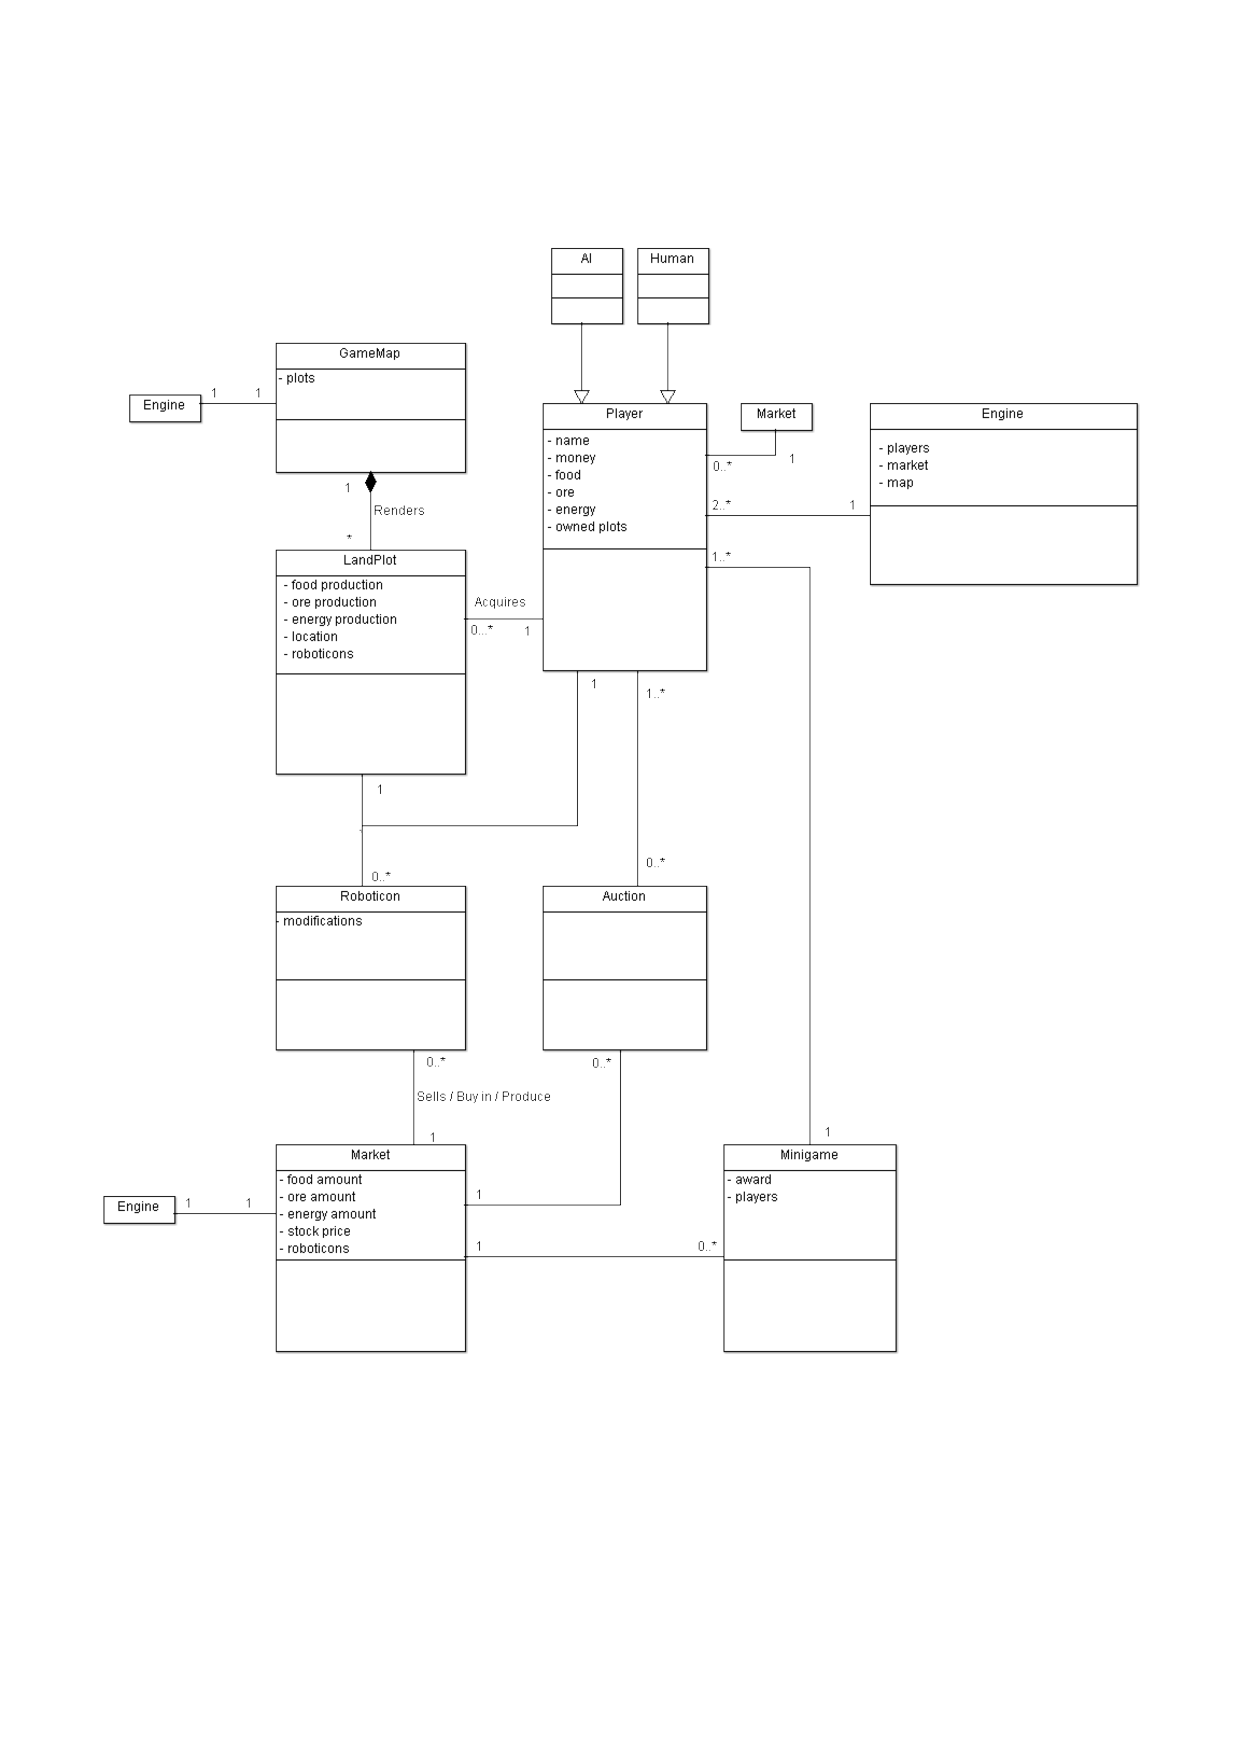
\includegraphics{AbstractDiagram.pdf}
		\caption{Abstract UML class diagram showing the relationships between classes in the software}
		\label{fig:classdiagram}
	\end{centering}
\end{figure}

\subsection{Entities}
We have identified the following classes that will be used in our system: \\

\begin{tabular}{|l|p{13cm}|}
	\hline
	Engine & The game engine itself, in charge of communications between classes. \\ \hline
	Player & The player entity has 2 child classes - AI and Human. Both have same base method and property names, with some different method bodies. \\ \hline
	LandPlot & Each instance of this class will represent a single tile on the map \\ \hline
	GameMap & This class is controlled directly from the engine. It stores all “LandPlot” instances. \\ \hline
	Roboticon & Roboticon is used in LandPlot for resource generation, trade between the player and the market. \\ \hline
	Market &The trading center. Players can buy or sell different types of resources and roboticons. It connects with the minigame class. \\ \hline
	Minigame & This class content a minigame for gambling, it is connected to the Market. \\ \hline
	Auction & The auction system, each instance will handle an individual auction that involves specific or selected players. \\ \hline
	
\end{tabular}

\subsection{Collaboration Diagrams}
These are collaboration diagrams which show how the classes in our game will interact to complete various tasks.
They also allowed us to test our class diagram and ensure that all necessary relationships had been established.
They are provided as Figures~\ref{fig:collab1}~to~\ref{fig:collab8}.

\begin{figure}[h]
	\begin{centering}
		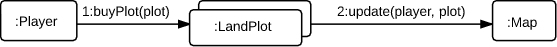
\includegraphics[width=\textwidth]{figures/collab1.png}
		\caption{Collaboration Diagram: Buying a plot of land}
		\label{fig:collab1}
	\end{centering}
\end{figure}
\begin{figure}
	\begin{centering}
		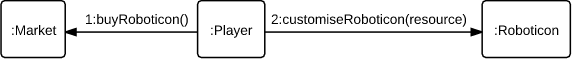
\includegraphics[width=\textwidth]{figures/collab2.png}
		\caption{Collaboration Diagram: Buying/Customising Roboticon from Market}
		\label{fig:collab2}
	\end{centering}
\end{figure}
\begin{figure}
	\begin{centering}
		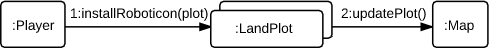
\includegraphics[width=\textwidth]{figures/collab3.png}
		\caption{Collaboration Diagram: Roboticon Installation}
		\label{fig:collab3}
	\end{centering}
\end{figure}
\begin{figure}
	\begin{centering}
		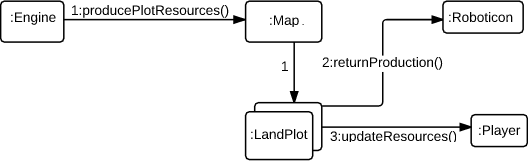
\includegraphics[width=\textwidth]{figures/collab4.png}
		\caption{Collaboration Diagram: Production of Resources}
		\label{fig:collab4}
	\end{centering}
\end{figure}
\begin{figure}
	\begin{centering}
		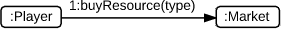
\includegraphics[]{figures/collab5.png}
		\caption{Collaboration Diagram: Buying from Market}
		\label{fig:collab5}
	\end{centering}
\end{figure}
\begin{figure}
	\begin{centering}
		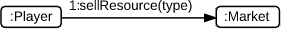
\includegraphics[]{figures/collab6.png}
		\caption{Collaboration Diagram: Selling to Market}
		\label{fig:collab6}
	\end{centering}
\end{figure}
\begin{figure}
	\begin{centering}
		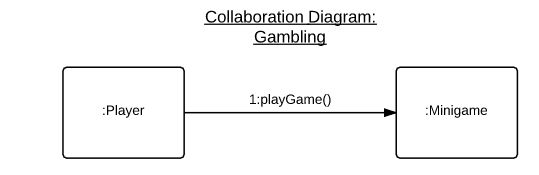
\includegraphics[]{figures/collab7.png}
		\caption{Collaboration Diagram: Gambling}
		\label{fig:collab7}
	\end{centering}
\end{figure}
\begin{figure}
	\begin{centering}
		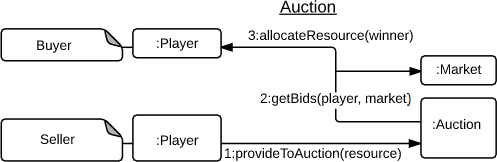
\includegraphics[width=\textwidth]{figures/collab8.png}
		\caption{Collaboration Diagram: Auction}
		\label{fig:collab8}
	\end{centering}
\end{figure}


\section{Systematic Justification of Architecture}
Designing an abstract representation of the system architecture required a lot of thought from the team, as it is easy to overlook important relationships between classes and objects.
We began the design process by looking through the brief and our requirements document and creating a list of classes that we felt encompassed the fundamental game elements.
From this process, we came up with the entities shown in the table above.
Below is a description of how each class will work and justification for why it will work that way.

\subsection{Engine}
The game engine is a particularly important class, as it is responsible for initiating and controlling each phase of the game, as well as invoking random events which will affect the game’s current state. In order for the Engine to be able to do this, it must be able to communicate with the other fundamental classes, these being the GameMap and each instance of the Player class.
From the brief, we established that there is a one-to-one relationship between the Engine and the GameMap, and a one-to-many relationship between the Engine and the Player (we have set the number of instances of player to be two at the moment). The Engine doesn’t need to be connected to other classes such as the Market and the LandPlot as these can be accessed via GameMap and Player.
We chose not to give many classes a relationship with the Engine, as this will create too many class couplings, meaning that if we need to make changes in the Engine class, changes will need to be made in many other classes too.

\subsection{Player}
The player class models each player in the game, and the set of decisions that they can make while playing.
These decisions include: buying plots of land, installing roboticons on plots, buying and selling from the market, and gambling in the bar (as detailed throughout the requirement section).
Because of the player’s large range of actions in the game, we needed the player to have relationships with quite a few of the other classes, including the Market, the Auction, various instances of the LandPlot class, and the Minigame.
Although this may seem risky due to the slightly monolithic nature of the class, we feel that the only way we can deliver a piece of software which satisfies all of the requirements is to design the system in this way.
The Player class will be the parent of two other classes called Human and AI.
These classes will inherit the attributes and methods of player, but will overwrite methods to suit each player role.
The player will have attributes detailing the name of the player, as well as the amount of money they have, the number of each resource they own (food, energy, ore), and the plots they own.

\subsection{Roboticon}
The roboticon class is responsible for production of resources on a plot, as stated in requirement 7.1.1., and any modifiers that will be applied to the rate of production.
It is therefore necessary for a roboticon to be able to communicate with the land plot on which it is placed.
In accordance with requirements 6.1.4. and 6.1.5. the player will be able to customise the roboticon by installing upgrades for money.
Finally the roboticon is produced, stored, and sold by the market so the classes must be able to communicate, as described in requirements 6.1.1 and 6.1.2..
It will have attributes to determine how it will alter the production of resources on a plot.

\subsection{Market}
The Market is the class responsible for managing the price of resources in the game (based on supply and demand), and also producing roboticons, as specified in requirement 8.1.2..
The player can directly buy and sell resources to/from the market so must be able to interact with it.
The market will also engage in the auction, placing bids against the other player and affecting the price at which resources are bought and sold. It will therefore interact with the auction.
The market also has a relationship with roboticons as it can buy sell and produce them.

\subsection{Minigame}
The minigame is a fairly simple class as it only interacts with the player.
The minigame is a game found in the market which will allow the player to gamble and either gain or loses money which will satisfy requirement 9.1.1.

\subsection{Auction}
The Auction Class is responsible for players buying and selling resources to each other, as described in requirement 8.1.1.
The market will also act as a bidder in the auction giving bids based on the supply/demand of the resource allowing access to the auction in a 2 player Game.
The auction will take resources to be sold from one player and bids from the other player(s) and the market, then provide the resources to the highest bidder.

\subsection{LandPlot}
The LandPlot class is used for purchase, resource production and customisation as Player request as described in requirement 2, 7.1.3 and 3.1.1.
All LandPlots instances are stored inside the GameMap class for rendering, and those LandPlots shall have the same size as described in requirement 1.2.2.
On the occurrence of random event, the production rate for different resources should change respectively if criteria matches per requirement 2.2.2. 

\subsection{GameMap}
The GameMap Class is in charge of storing all instances of LandPlot and the interaction with the Engine to render the Game Map to the screen.
At beginning of the game, GameMap will initialise and set all LandPlots to a state of “unoccupied” to allow the Player to view and purchase as described on requirement 1.1.1 and 2.2.3.



\chapter{Method Selection and Planning}
\section{Outline and Justification of Software Engineering Methods and Tools}

Choosing a set of software engineering methods for our SEPR project has required careful consideration from us as a team.
Many factors can influence the suitability of certain methods for a project, such as team size, the type of system being delivered and the volatility of user requirements.
It was through the analysis of these type of factors that we came to a decision about which methods we would be using.

A key aspect of a software engineering method is its development lifecycle, which dictates and characterises each engineering activity.
Many different lifecycles exist, with varying characteristics, so it was important for us to explore some different types and decide which one was best for our project.
We decided that methods based on an incremental development lifecycle would be most suited to us, as it protects us against volatile requirements and allows us to regularly get feedback from our customer.
This means we can produce an end result which is as close to our customers expectations as possible. We explored alternative lifecycles to the incremental approach, including the “waterfall” approach proposed by Winston Royce~\cite{royce1970managing}.
We discarded this approach however because the model struggles to deal with changes of requirements, and also has large documentation overheads which are not necessary for the size of our project.
There is also risk involved with this model as the first time the customer sees the software is at the end of the lifecycle, so if they are not satisfied then it will be very hard to fix broken procedures and implement new ones.

Now that we had decided on our development lifecycle, we next had to decide on a set of engineering methods and principles which fit the incremental approach.
Once again, there are a large number of methods which fit this approach so an investigation of these methods and their differences was required.

We looked at the Rational Unified Process (RUP) proposed by Rational, now a division of IBM, which is a plan-based incremental engineering method.
RUP splits each iteration of the development lifecycle into four phases, called the inception phase, elaboration phase, construction phase and transition phase.
Each phase has a well defined milestone which is achieved at the end of the phase~\cite{rup1998}.
The first two phases involve the creation of a requirements list, use cases, risk assessments, project plans, a system architecture amongst other planning phase documents.
The next two phases are all about the development, testing and integration of the system into the customer’s working environment.
After evaluation and consideration, we decided that RUP wouldn’t be best suited to our project.
The problem we found was that in order to use this development process, you need strong knowledge from the outset of how the system will work in order to develop the use cases.
While we have been given a brief, from interviewing our customer we discovered that certain features have been left up to us to develop, meaning that working through the first two phases of RUP in each lifecycle would be difficult and cost us time, leaving us with less time to actually develop the software.
Also, according to Boehm, “only change rates on the order of 1\% of the requirements are acceptable” for plan-based development~\cite[p 31]{boehm2003balancing}.
With our project, requirements may change on a regular basis, meaning that this approach may not be able to cope.

We decided instead to adopt an Agile approach to the software engineering of this project due to its merging of design and implementation phases and short iteration lifecycles which will allow the system to organically grow as we incorporate customer feedback into the development process. We will mainly be following the eXtreme Programming (XP) and Scrum agile methods, as the principles in each method work very well for small teams who can stay in regular contact with their customer, which is perfect for us. Some of the principles from the eXtreme Programming agile method that we will be using in the development of our project are:
\begin{itemize}
	\item Test Driven Development (TDD)
	\item Refactoring
	\item Incremental Planning \& User Stories
	\item Pair Programming
	\item Small releases \& updates of the final product~\cite{sommerville2016software}
\end{itemize}

In order to write code and collaborate as a team, we are going to need a version control system.
Git seems like a suitable option, as it allows us to work on different sections of code together in local repositories before committing updates to the main repository without blocking each other's productivity.
A good team also requires good communication, so we will be using the Slack service as it allows us to talk on multiple channels, and integrate other services into conversations (e.g. Git commits and updates).
Organising tasks which need to be completed is another important part of collaboration, and Trello provides a very nice way of doing this.
We can set up different “cards” on a Trello dashboard for different backlogs of task, meaning that we always know what needs to be completed, what is being completed and what has been completed.

\section{Team Organisation}

Team organisation can be the difference between a successful project and a failure, so we took the time to choose an approach to organisation which will allow the team to collaborate effectively, and reflect on improvements we need to make as a team in order to be successful.
The Scrum methodology seems like an excellent way to organise the team, and fits in well with the other Agile methods and principles we are using e.g. user stories from eXtreme Programming~\cite{sommerville2016software}.

We will begin each iteration of our software lifecycle by reviewing our current user stories and breaking them down into tasks which can then be implemented into the system.
Test cases can also be generated from these stories for Test Driven Development.
We will have a Trello dashboard with cards for the Product Backlog and the Sprint Backlog where all the tasks and the current sprint tasks respectively will be stored, allowing us to move tasks from the left to the right as they are completed by the team.
Once the tasks we are completing during the sprint have been established, we will carry out the sprint which will last for around 4 - 5 days.
During this time we will attempt to implement as many of the tasks in the Sprint Backlog as we can, as well as having a regular meeting each day called a Scrum where we say what we are working on, how we are getting on with it, and if we are having any issues.
After the sprint is finished, we should ideally have a version of our system that is working and includes all of the functionality we have implemented so far.
We will then have a sprint review, where we discuss how the sprint went, if there is any outstanding functionality which wasn't implemented during the sprint and if there are any ways in which we can improve team productivity. 

\section{Project Plan}

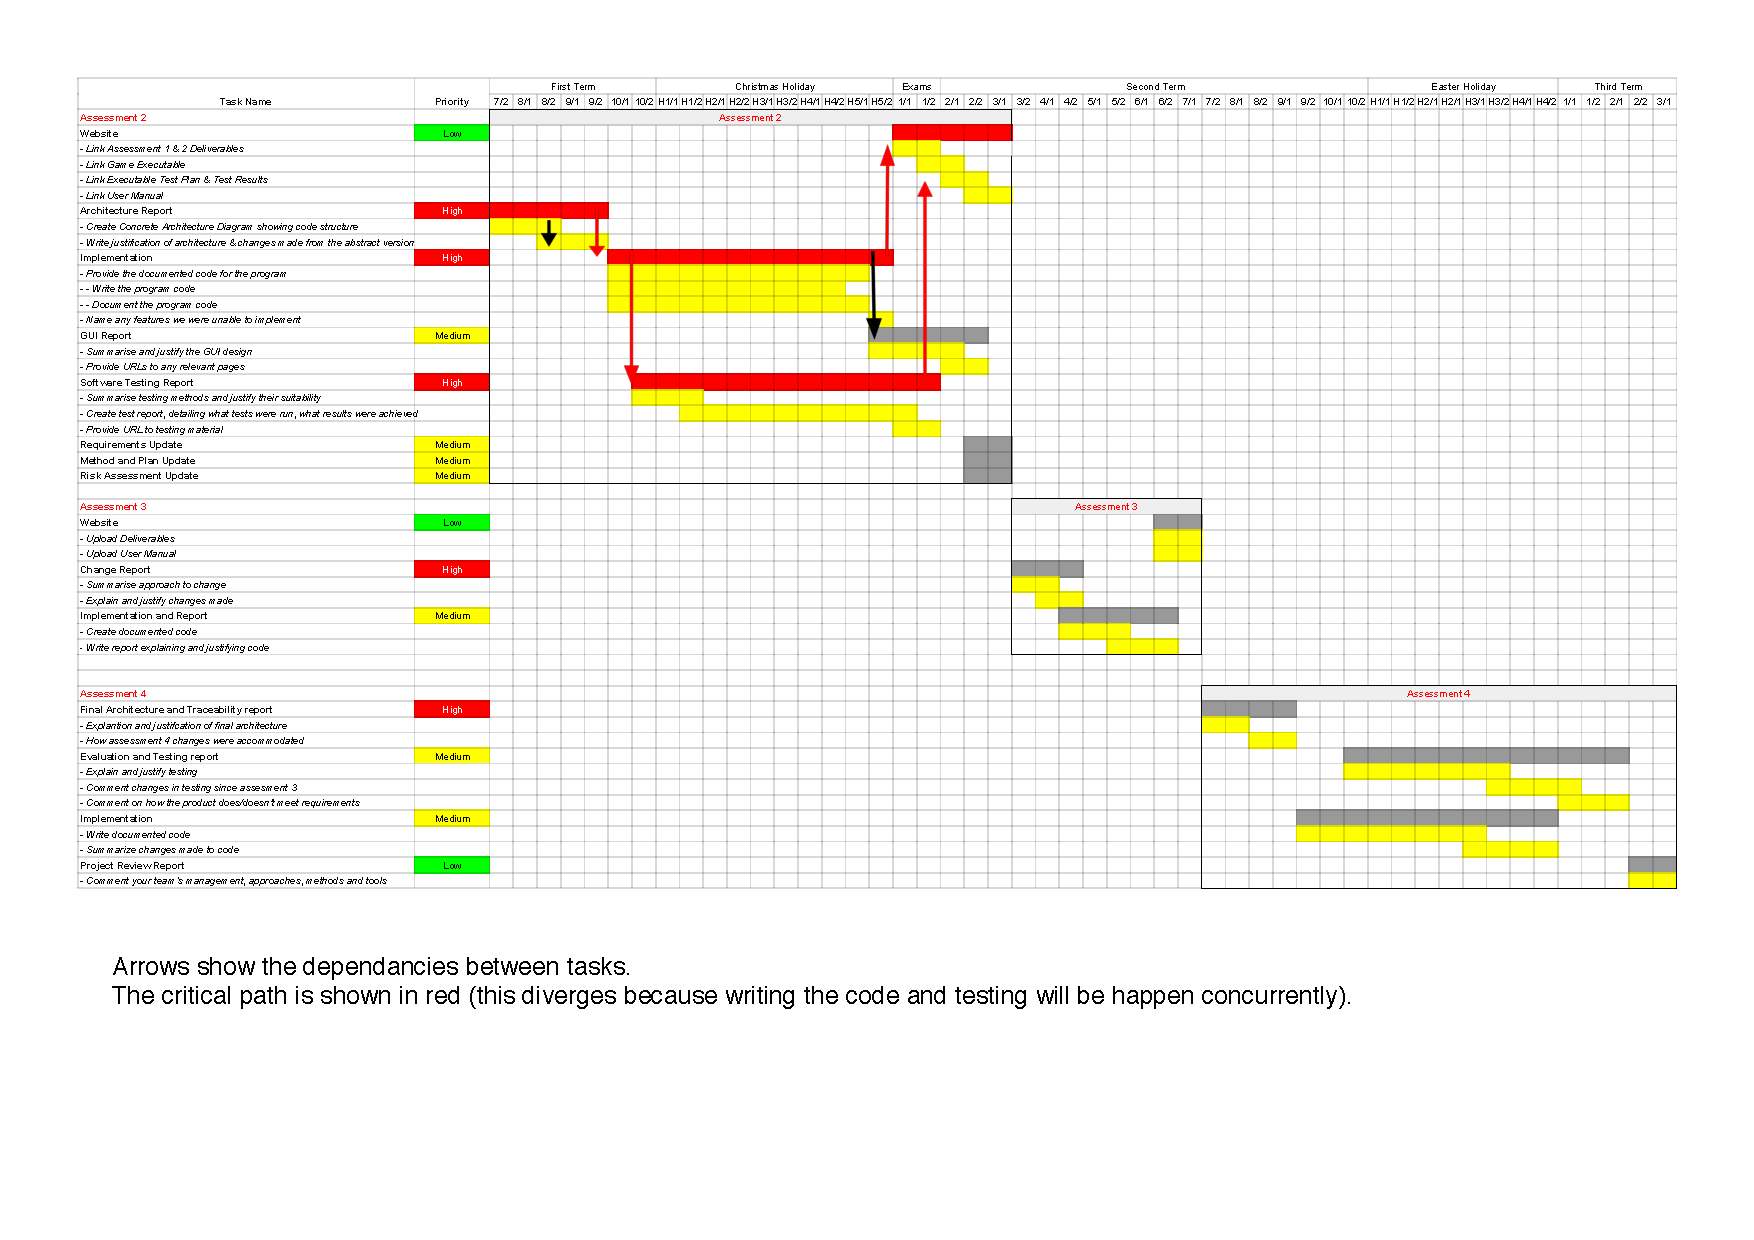
\includepdf[pages=1, landscape=true]{plan.pdf}

\bibliographystyle{ieeetr}
\bibliography{references.bib}

\chapter{Risk Assessment and Mitigation}
\section{Introduction}
Throughout the project we will face a number of potential risks however we will do our best to mitigate them.
When analysing the risks we will focus on two factors, likelihood and severity.

A risk can either have a high, medium, or low chance of becoming a reality.
If a problem is not likely to occur when running a project three times or more we deem it to have a low likelihood.
If it is likely to occur once during the project or when running a project twice we deem it medium likelihood.
Finally, if it is likely to occur multiple times during the project, we will deem it as high likelihood.

A risk can also either be high, medium, or low in severity.
A high severity risk could result in months of lost progress up to having to totally start over.
A medium severity risk could result in the loss of between one week and a few weeks of progress.
Finally a low severity risk would only result in a maximum of a few days of lost progress.

To combine these two factors into something meaningful we will use a risk matrix (Figure~\ref{fig:risktable}).
This will allow us to find a balance and identify the risks that will pose major problems.

\begin{figure}[h]
	\centering
	\begin{tabular}{|l|l||l|l|l|}
		\hline
		\multicolumn{2}{|l||}{\multirow{2}{*}{}} & \multicolumn{3}{c|}{Likelihood} \\ \cline{3-5}
		\multicolumn{2}{|l||}{}                  & Low       & Medium   & High     \\ \hhline{|==||=|=|=|}
		\multirow{3}{*}{Severity}    & Low      & Low       & Low      & Medium   \\ \cline{2-5}
		& Medium   & Low       & Medium   & High     \\ \cline{2-5}
		& High     & Medium    & High     & High     \\ \hline
	\end{tabular}
	\caption{Table showing how likelihood and severity of a risk combine to show overall impact of the risk}
	\label{fig:risktable}
\end{figure}

Green cells in the matrix are considered to be overall low risk, this is because they are not particularly likely to happen and if they do they will not have be severe enough to majorly impact the project.
Orange cells signify an overall medium risk.
They are either likely to happen but low severity, very unlikely to happen but would have a very severe impact or somewhere between.
Overall high severity risks, red cells, are the most important to mitigate.
They have a reasonably high chance of happening and could result in the loss of weeks or months of work.

It is important to categorise risks once they have been identified so that we can prioritise mitigation, it is imperative that overall high risks cannot happen and in the case that they do we must be able to cope with them and have protocols in place to lessen the impact.

We will be presenting the risks in a risk register with columns identifying, analysing and showing the mitigations for the risk.
This will give us an accessible and easily modifiable document which we will be able to use throughout the project when considering or attempting to mitigate risks.

\newpage

\begin{landscape}
\section{Risk Assessment}
\begin{longtable}{|l|p{5cm}|l|l|l|p{4cm}|p{5cm}|}
	\hline
	\textbf{Category} & \textbf{Name} & \textbf{Severity} & \textbf{Likelihood} & \textbf{Overall} & \textbf{Mitigation} & \textbf{Contingency} \\ \hline \hline
	\endhead
	Staff & Team member leaves & High & Low & Medium & & \\ \hline
	Staff & Staff sick or unable to attend meetings. & Medium & High & High & Let other members of the team know as soon as possible & Other staff takes over their work temporarily. \\ \hline
	Staff & Don’t have the skill required to complete the task. & Low & Medium & Low & Research the skills needed. Ask other team members if they know how to help. & Read books and the internet about required skills. \\ \hline
	Staff & Staff don’t listen others opinion& Low & Low & Low & More communication, consult Richard/Fiona if the problem continues. & Stay together and work out the root reason, then resolve it. \\ \hline
	
	Staff/Requirements & Staff failed to complete the task before deadline. & High & Low & Medium & More rapid sprint to ensure everyone is on track. & Cut our optional features and complete the compulsory requirements first. \\ \hline
	
	Requirements & Change of requirements & Low & High & Medium & Keep in touch, build and show to the client & Update the requirement document and update the product. \\ \hline
	Requirements & Responsible of telling the customer that requirements were impossible and offer alternative options. & Low & Low & Low & Negotiate with the customer before updating the requirements. & Explain to the customer what has to be changed. \\ \hline
	Requirements & Cannot meet the requirement & High & Low & Medium & Design realistic requirements before start coding. & Modify the requirements so it can be met. \\ \hline
	
	Tech & Data lost - e.g. hard drive failure. & Medium & Low & Low & Backup data regularly to cloud or different devices. & Restore most recent backed up data. \\ \hline
	Tech & IT facility failure & Low & Low & Low & Routine maintenance to devices. & Use campus computer to continue development. \\ \hline
	Tech & Security threats & High & Low & Medium &  Install antivirus software and enable firewall. & Seek IT support for help and continue working. \\ \hline
	Tech & Software bug that causes data loss. & High & Medium & High & Backup data before executing dangerous commands. & Reset to the previous commit using git. \\ \hline
	
	Tools & Tools not available & Low & Medium & Low & Research background information about alternatives before proceeding. & Switch to an alternative tool, request help from IT support or create one if enough time before deadline. \\ \hline
	Tools & Unfamiliar with the toolset. & Low & Medium & Low & Learn how to use the tool. & Ask IT support or other teammates for help. \\ \hline
	Tools & Tools does not fit into the project after start off. & Low & Medium & Low & Do extensive research and comparison before integrating to the workflow. & Find alternative and re-evaluate options. \\ \hline
	
	Estimation & Estimates that there will not be enough time to finish the whole project. & High & Medium & High & Allocate and plan the time efficiently. & Plan and spend more time for the project. \\ \hline
	
	Customer & Customer changes the requirements. & Low & High & Medium & Keep in touch and understand the necessary changes as soon as possible. & Examine new requirements and update them accordingly. \\ \hline
	Customer & Customer doesn't allow or understand why we have to change the requirements. & Medium & Medium & Medium & Keep in touch with the customer & Sit next with the customer and talk through the reason why. \\ \hline
	
	Test & Bugs discovered & Medium & High & High & Understand the code and have comments around them. & Fix bugs. \\ \hline
	Test & Something wrong but cannot find the errors. & Medium & Medium & Medium & Put comment around the code to describe, and do tests. & Debug the problem using a debugger and seek for help. \\ \hline
	
\end{longtable}
\end{landscape}

\end{document}  